\documentclass[aspectratio=169]{beamer}
\usetheme{Madrid}
\usepackage[utf8]{inputenc}
\usepackage[T1]{fontenc}
\usepackage{tikz}
\usepackage{amssymb}
\usepackage{graphicx}
\setbeamertemplate{navigation symbols}{}
\setbeamercolor{title}{fg=white,bg=orange!85!red}
\setbeamercolor{frametitle}{fg=white,bg=orange!85!red}
\setbeamercolor{block title}{bg=orange!85!red!20,fg=black}
\setbeamercolor{block body}{bg=orange!85!red!8,fg=black}
\setbeamercolor{item}{fg=orange!85!red}
\setbeamercolor{itemize item}{fg=orange!85!red}
\setbeamertemplate{itemize item}[triangle]

\title{Web Story 3 — Remembering After You Leave}
\subtitle{localStorage — data that survives a page refresh}
\author{ByteForge --- Grade 8 --- App Builder}
\date{}

\begin{document}

\begin{frame}
    \titlepage
\end{frame}

\begin{frame}{Today's Plan}
    \begin{itemize}
        \item Remember After Refresh
        \item Save the Whole Inventory
        \item Was Anything Saved Before?
        \item[$\bigstar$] BOSS --- A Story That Remembers You
    \end{itemize}
\end{frame}

\begin{frame}{localStorage genuinely survives a refresh}
    \large
    \begin{itemize}
        \item Every variable, array, and object used so far disappears the instant the page reloads. localStorage is different
        \item Saved to the browser itself, still there after closing the tab entirely.
    \end{itemize}
\end{frame}


\begin{frame}{localStorage only holds TEXT}
    \large
    \begin{itemize}
        \item \texttt{JSON.stringify()} correctly turns a real array/object into text that can be perfectly reconstructed later; \texttt{JSON.parse()} reverses it exactly
        \item Same items, same order.
        \item Worked example: \texttt{JSON.stringify(["sword","shield"])} produces the text \texttt{'["sword","shield"]'} — and \texttt{JSON.parse()} on that text rebuilds the EXACT original array, not just something similar-looking.
    \end{itemize}
\end{frame}


\begin{frame}{null means "nothing was ever saved"}
    \large
    \begin{itemize}
        \item The very first time anyone visits a page, \texttt{localStorage.getItem()} returns null for everything
        \item Any real save system has to handle this "first visit" case explicitly.
    \end{itemize}
\end{frame}


\begin{frame}{BOSS — real persistent story state}
    \large
    \begin{itemize}
        \item Saving structured data, loading it back, and checking whether it existed first
        \item This is genuinely how real websites remember your cart, progress, or preferences between visits.
    \end{itemize}
\end{frame}

\begin{frame}{Real-World Examples}
    \large
    \begin{itemize}
        \item Every website that remembers your dark-mode preference or your shopping cart after you close the tab is using exactly this mechanism. Minecraft's own save files work on the same principle at a bigger scale
        \item Your world genuinely persists between sessions, saved to disk, not just held in memory while running.
    \end{itemize}
\end{frame}


\begin{frame}{Image}
    \begin{center}
    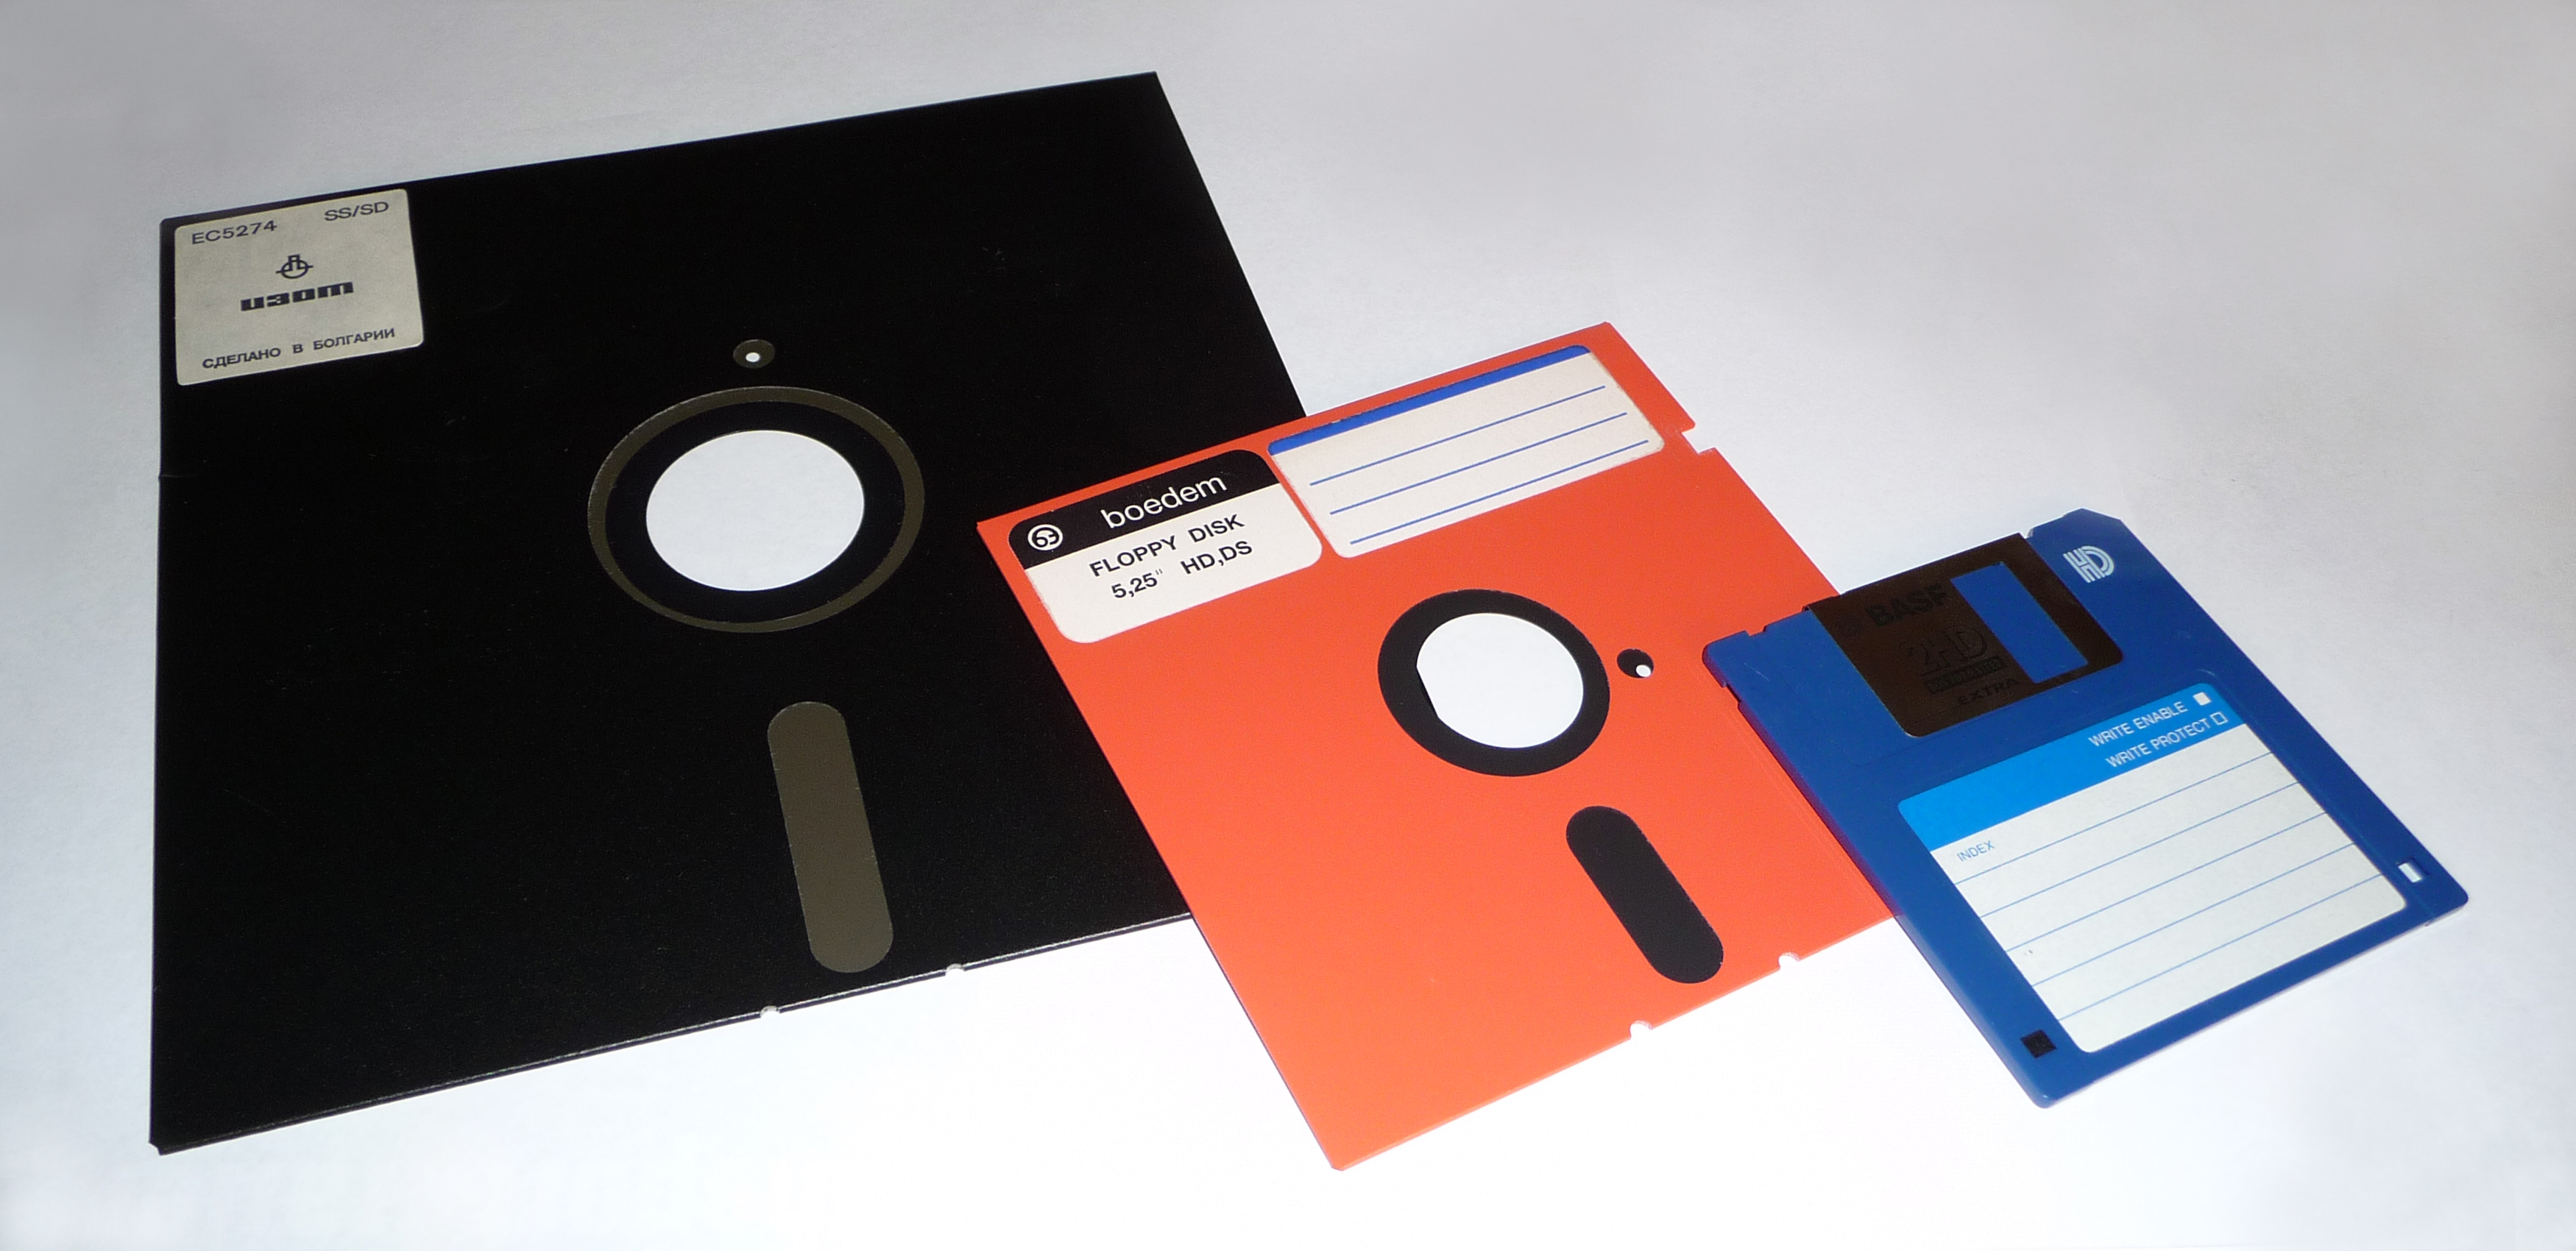
\includegraphics[width=0.5\textwidth]{images/floppy.jpg}

    \large Old-school 'save to disk' --- the exact idea localStorage recreates inside the browser.

    \small Floppy disks, George Chernilevsky, public domain, via Wikimedia Commons
    \end{center}
\end{frame}

\begin{frame}{Let Them Discover}
    \Large
    Close and reopen a website that remembers something about you (a cart, a login, a dark-mode setting). What do you think happens the very FIRST time anyone ever visits — before anything has been saved yet?
\end{frame}

\begin{frame}{Your Turn}
    \Large
    Open the student map, find \textbf{Web Story 3 — Remembering After You Leave}, and work through it
    hands-on --- everything you just saw, they now do themselves.
\end{frame}

\end{document}
